\documentclass{article}

\usepackage{dirtree}

\usepackage[
  height=9in,      % height of the text block
  width=7.5in,       % width of the text block
  top=78pt,        % distance of the text block from the top of the page
  headheight=48pt, % height for the header block
  headsep=12pt,    % distance from the header block to the text block
  heightrounded,   % ensure an integer number of lines
        % show the main blocks
  verbose,         % show the values of the parameters in the log file
]{geometry}
\setlength{\parindent}{0pt}
\usepackage{amsmath}
\usepackage{courier}
\usepackage{graphicx}
\usepackage{amsmath}
\usepackage{booktabs}
\usepackage{fancyhdr}
\usepackage{float}
\usepackage{mathtools}

\pagestyle{fancy}
\fancyhead[L]{Pattern and Speech Recognition WS1617\\ Assignment 08}
\fancyhead[R]{ Vinh Thinh Ho (2562630) \\ Noshaba Cheema (2562653)}

\renewcommand{\headrulewidth}{0.35pt}
\newcommand\tab[1][1cm]{\hspace*{#1}}

\begin{document}
\section*{Exercise 8.1}
a)\\
\begin{align*}
s1[t] &= (f*k)[t]\\
&= f[t] * k[0] + f[t-1] * k[1] = \frac{1}{2}(f[t] + f[t-1])
\end{align*}
Hence, $s1 = \frac{1}{2}[3, 1 + 3, 8 + 1, 6 + 8, 3 + 6, 9 + 3, 5 + 9, 1 + 5, 1] = [1.5, 2, 4.5, 7, 4.5, 6, 7, 3, 0.5]$\\
b)\\
The same we have:
\begin{align*}
s2 &= s1 * k\\
&= [0.75, 1.75, 3.25, 5.75, 5.75, 5.25, 6.5, 5, 1.75, 0.25]
\end{align*}
c)
\begin{figure}[ht]
\centering
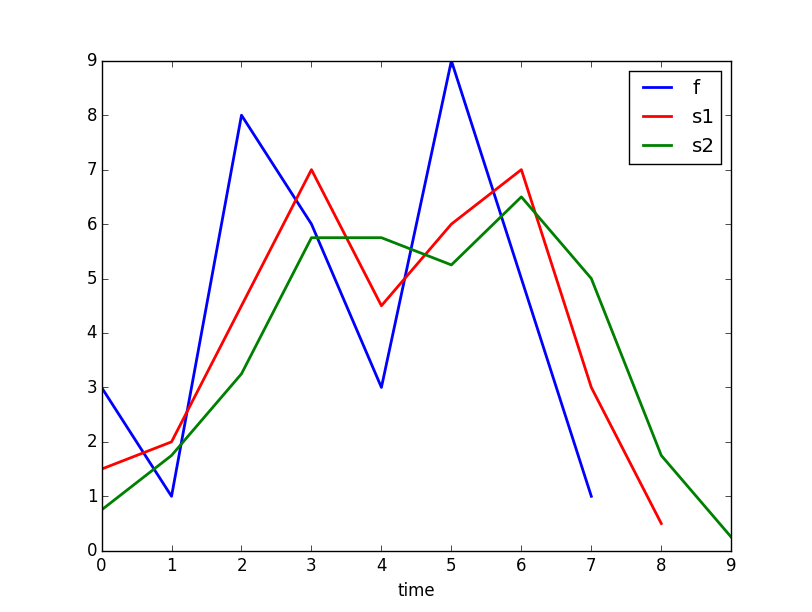
\includegraphics[scale=0.5]{81c.png}
\end{figure}\\
- Convolving f for n times with n $\to \infty$, the resulted signal would be averaged and be closed to zero. With n $= \infty$, the resulted signal would be 0.\\
d)
\begin{align*}
k' &= k * k = [0.25, 0.5, 0.25]\\
s3 &= f * k' = [ 0.75,  1.75,  3.25,  5.75,  5.75,  5.25,  6.5 ,  5.  ,  1.75,  0.25]
\end{align*}
e)\\
We can see that s2 = s3. This is due the associative property of convolution: $s2 = (f * k) * k = f * (k * k) = s3$\\
Proof:  given arbitrary signal $a, b, c$, we have:
\begin{align*}
((a * b) * c)[t] &= \sum\limits_{i} (a*b)[i].c[t-i]\\
&= \sum\limits_{i}\sum\limits_{j}a[j].b[i-j].c[t-i]\ \ \ \ \ (1)
\end{align*}
And:
\begin{align*}
(a * (b * c))[t] &= \sum\limits_{x} a[x].(b*c)[t-x]\\
&= \sum\limits_{x} a[x].\sum\limits_{y}b[y].c[t-x-y]\\
&= \sum\limits_{x}\sum\limits_{y}a[x].b[y].c[t-x-y]\ \ \ \ \ (2)
\end{align*}
Because $y$ is only dependent on $x$, we can set $x = j$ and $y = i - j$. Now we have:
\begin{align*}
a[x].b[y].c[t-x-y] &= a[j].b[i-j].c[t-j-(i-j)]\\
&= a[j].b[i-j].c[t-i]\ \ \ \ \ (3)
\end{align*}
From (1), (2) and (3) $\to$ \textbf{Proved}
\section*{Exercise 8.2}
b) See \textbf{82.py}\\
\begin{figure}[ht]
\centering
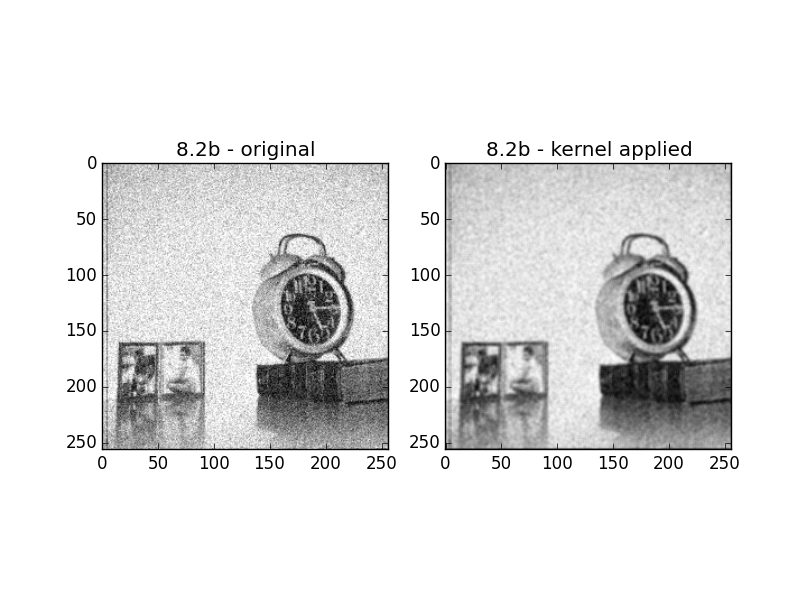
\includegraphics[scale=0.75]{blur.png}
\end{figure}
The kernel will average each image point with 8 surrounding, the effect is the image will be blurred. Image will be denoised when the kernel is applied.\\
c) See \textbf{82.py}\\
\begin{figure}[ht]
\centering
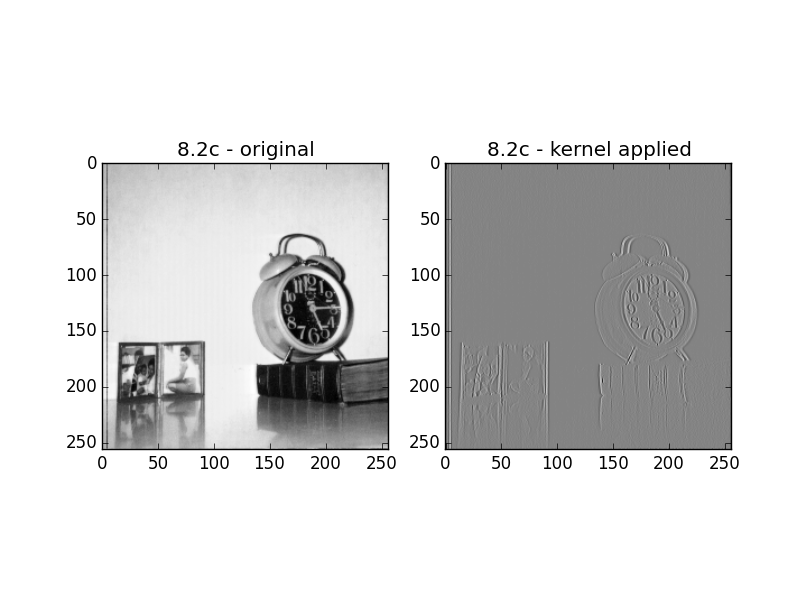
\includegraphics[scale=0.75]{82c.png}
\end{figure}
Applying this kernel, each point would be the difference between it and its 2 horizontal neighbor points . One application of this kernel is edge detection.\\
d)\\
The padding zero is not always optimal. For example, if the boundary have is dark (high gray value), one of it neighbor is also almost dark (because 2 neighbor points often have close values), the other neighbor is the padding would have value 0. After applying kernel, this point would have very negative value (always become light after rescaling), so it is less informative. A better padding is we can pad each point with a random point inside the image, or we could pad each point with the average value of points inside the image.
\newpage
\section*{Exercise 8.3}
See \textbf{83.py}\\
We trained using half of MNIST data, with only 1 epoch, using $batch\_size = 50$, and we vary the size of second hidden layer: 128, 256, 512, 1024. Below is the result:
\begin{figure}[ht]
\centering
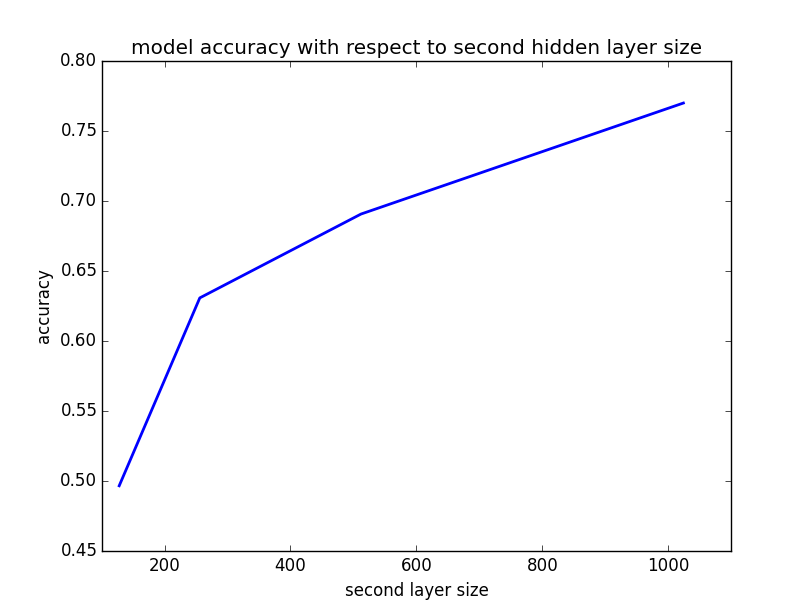
\includegraphics[scale=0.5]{83.png}
\end{figure}

We can see that when increasing the size of the second hidden layer, the accuracy of the model also increases.
\section*{Exercise 8.4}
\end{document}



